\documentclass[12pt]{article}
\usepackage[utf8]{inputenc}
\usepackage{cite}
\usepackage{graphicx}

\title{Smart and Efficient Techniques for Automated Guided Vehicle}
\author{Team ID 11, eYIC 19-20}
\date{December 2019}

\begin{document}

\maketitle

\section*{Keywords}
eYIC 19-20, SDG, AGV, Machine Vision, PCB, Versatile, Path Planning, Self  Charging, Remote Accessing

\section{Introduction}

Today the automated guided vehicle (AGV) plays an important role in the design and growth of new factories and warehouses. It is a robot that follows markers or wires in the floor or uses vision or lasers.  In an automated process, AGVs are programmed to communicate with other robots to ensure the product is moved smoothly through the warehouse, whether it is being stored for future use or sent directly to shipping areas. Navigation of AGVs is performed through laser, magnetic tapes, machine vision. As per increasing technologies, industries lack adaptive AGVs. That means, AGVs with constant hardware and software upgrades. Lack of vision-based navigation in the AGVs, make them single task-oriented. So, here we are proposing the advanced version of machine vision-based smart automated guided vehicle which incorporates the ML algorithm and would be beneficial for predicting the failures/problem before time and increasing task efficiency and accuracy. The proposed AGV also contains self-charging and can predict the possible future working hours of it. This adaptive AGV is low-cost since it must eventually attract more industries from various fields. Deploying it for repetitive material handling tasks can also allow enterprises to save on labor costs and reassign staff on other essential tasks, such as enhancing customer satisfaction.

\section{Literature Survey}

The automated guided vehicle represents the progress of automation in the industrial field. The first AGV was brought to market in the1950s, by Barrett Electronics \cite{agv_wiki}. Later in 2001, Fujimoto, Tomoya, Jun Ota, Tamio Arai, Tsuyoshi Ueyama, and Tsuyoshi Nishiyama proposed a way of estimation positioning error with magnetic tape to attempt fixed model learning to prevent stationary error while AGV runs iteratively\cite{fujimoto2001}. After in 2006, the authors Vis, Iris FA specify more specific research perspectives in the design and control of AGV systems in distribution and transportation systems. It concluded that new analytical and simulation models need to develop for large AGV systems to overcome large computational time, NP-completeness, congestion, deadlock, and delays in the system and finite planning horizons\cite{iris2006}. According to the research, the global Automated Guided Vehicle (AGV) market size was valued at USD 2.49 billion in 2018 and is projected to expand at a CAGR of 15.8\% from 2019 to 2025”\cite{grandviewresearch_site}. 

\section{Hardware Requirements}

\begin{enumerate}
    \item ATmega2560 Board
    \item Arm Cortex A53 Board
    \item ESP8266 Board
    \item ATmega328p Board
    \item Logitech C270 Webcam
    \item Monster Moto Shield VNH2SP30 Motor Driver 14A (Peak 30A)
    \item Johnson Geared Motor-Grade A Quality-300RPM
    \item MPU-6050 3-Axis Accelerometer and Gyro Sensor
    \item XL4015 5A Step Down Adjustable Power Supply with LED Voltmeter
    \item 58mm Plastic Omni Wheel for Lego
\end{enumerate}

\section{Software Requirements}

\begin{itemize}
  \item Autodesk Fusion
  \item Autodesk Eagle
  \item MATLAB \& Simulink
  \item Arduino IDE
  \item Python IDE
\end{itemize}

\section{Implementation}

Automated guided vehicles are mainly used for the transfer of loads from one place to another in industries. The implementation of proposed AGV is represented using Six modules.

\begin{figure}[htp]
\centering
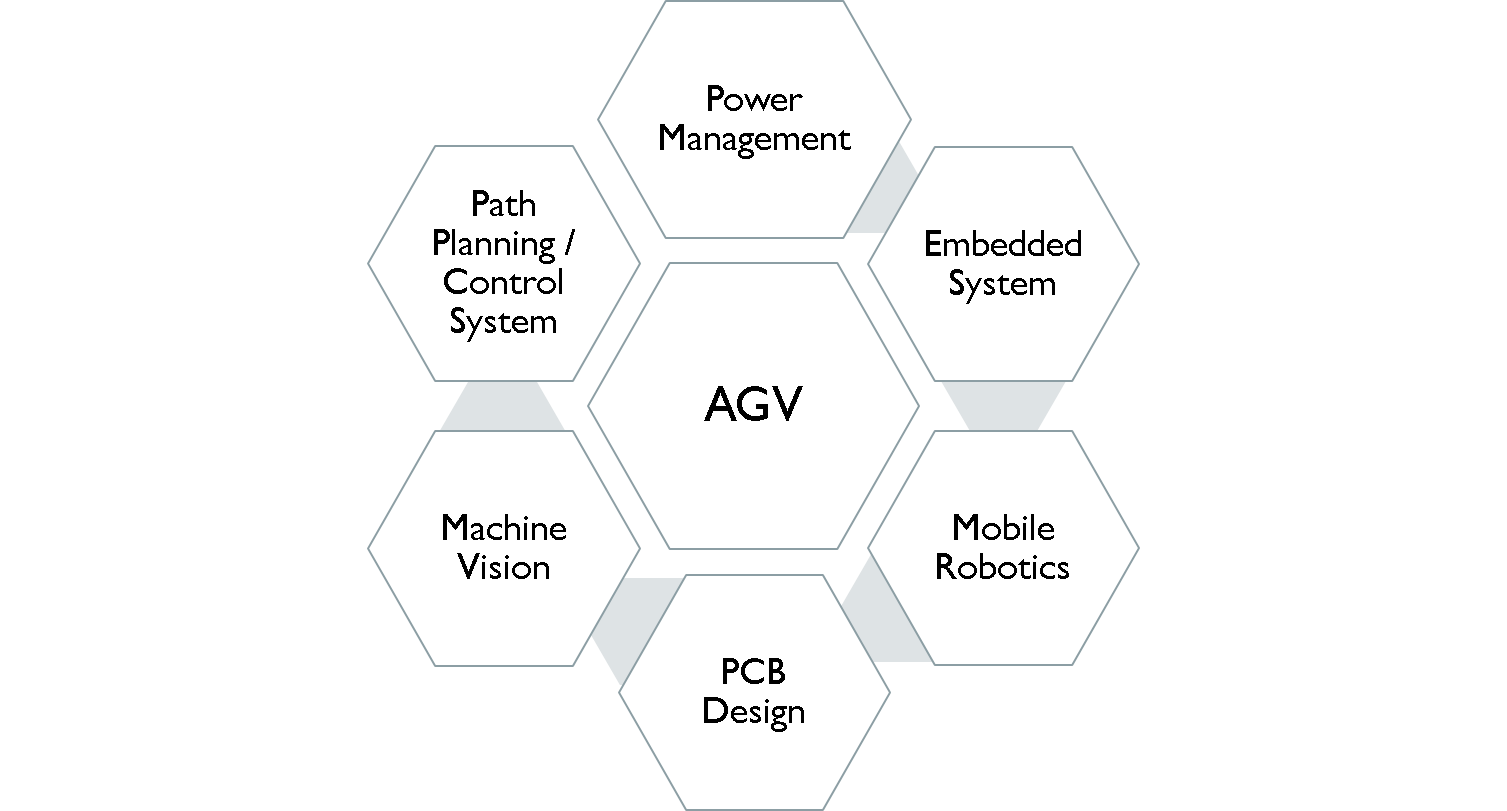
\includegraphics[width=15cm]{Modules.png}
\caption{Modules}
\label{fig}
\end{figure}

\begin{itemize}
  \item Power management: To make AGV more efficient the power management unit is integrated, which allows AGV to charge batteries without human interference. MCP 73831 IC is used for charging circuits and power management systems. It also regulates the voltage and current being provided for the whole circuitry of the AGV. Battery level can be indicated using LEDs for manual operation as well. This helps to increase productivity and save time.
  \item Embedded system: It includes ATmega 2660 controller board, Cortex A53 board, communication modules along with supportive software like Arduino IDE, Python IDE, Matlab, etc. Here, ATmega 2560 acts as a master controller. Data administration is done using the ESP8266 module and stored on the cloud.
  \item Pcb design: Self-designed PCB for AGV helps it to work in a multi-domain environment without major hardware changes. It performs power optimization and reduces circuitry. Each module has its own PCB board.
  \item Machine vision:  Machine vision operation is carried out using a web camera and cortex A53 controller board. A self-developed line following algorithm is used for navigation. It also performs obstacle avoidance and prevents occlusion.
  \item Path planning and control system: inertial measurement unit along with PID helps to keep AGV alined. IMU communicates with ATmega 2560 using the i2c bus. DC motor with 300rpm and 6kg-cm is controlled by a VNH2SP30 motor driver.

\end{itemize}
\newpage
\section{Flow Chart}

The working flow of the proposed automated guided vehicle is explained in the below flowchart.

\begin{figure}[htp]
\centering
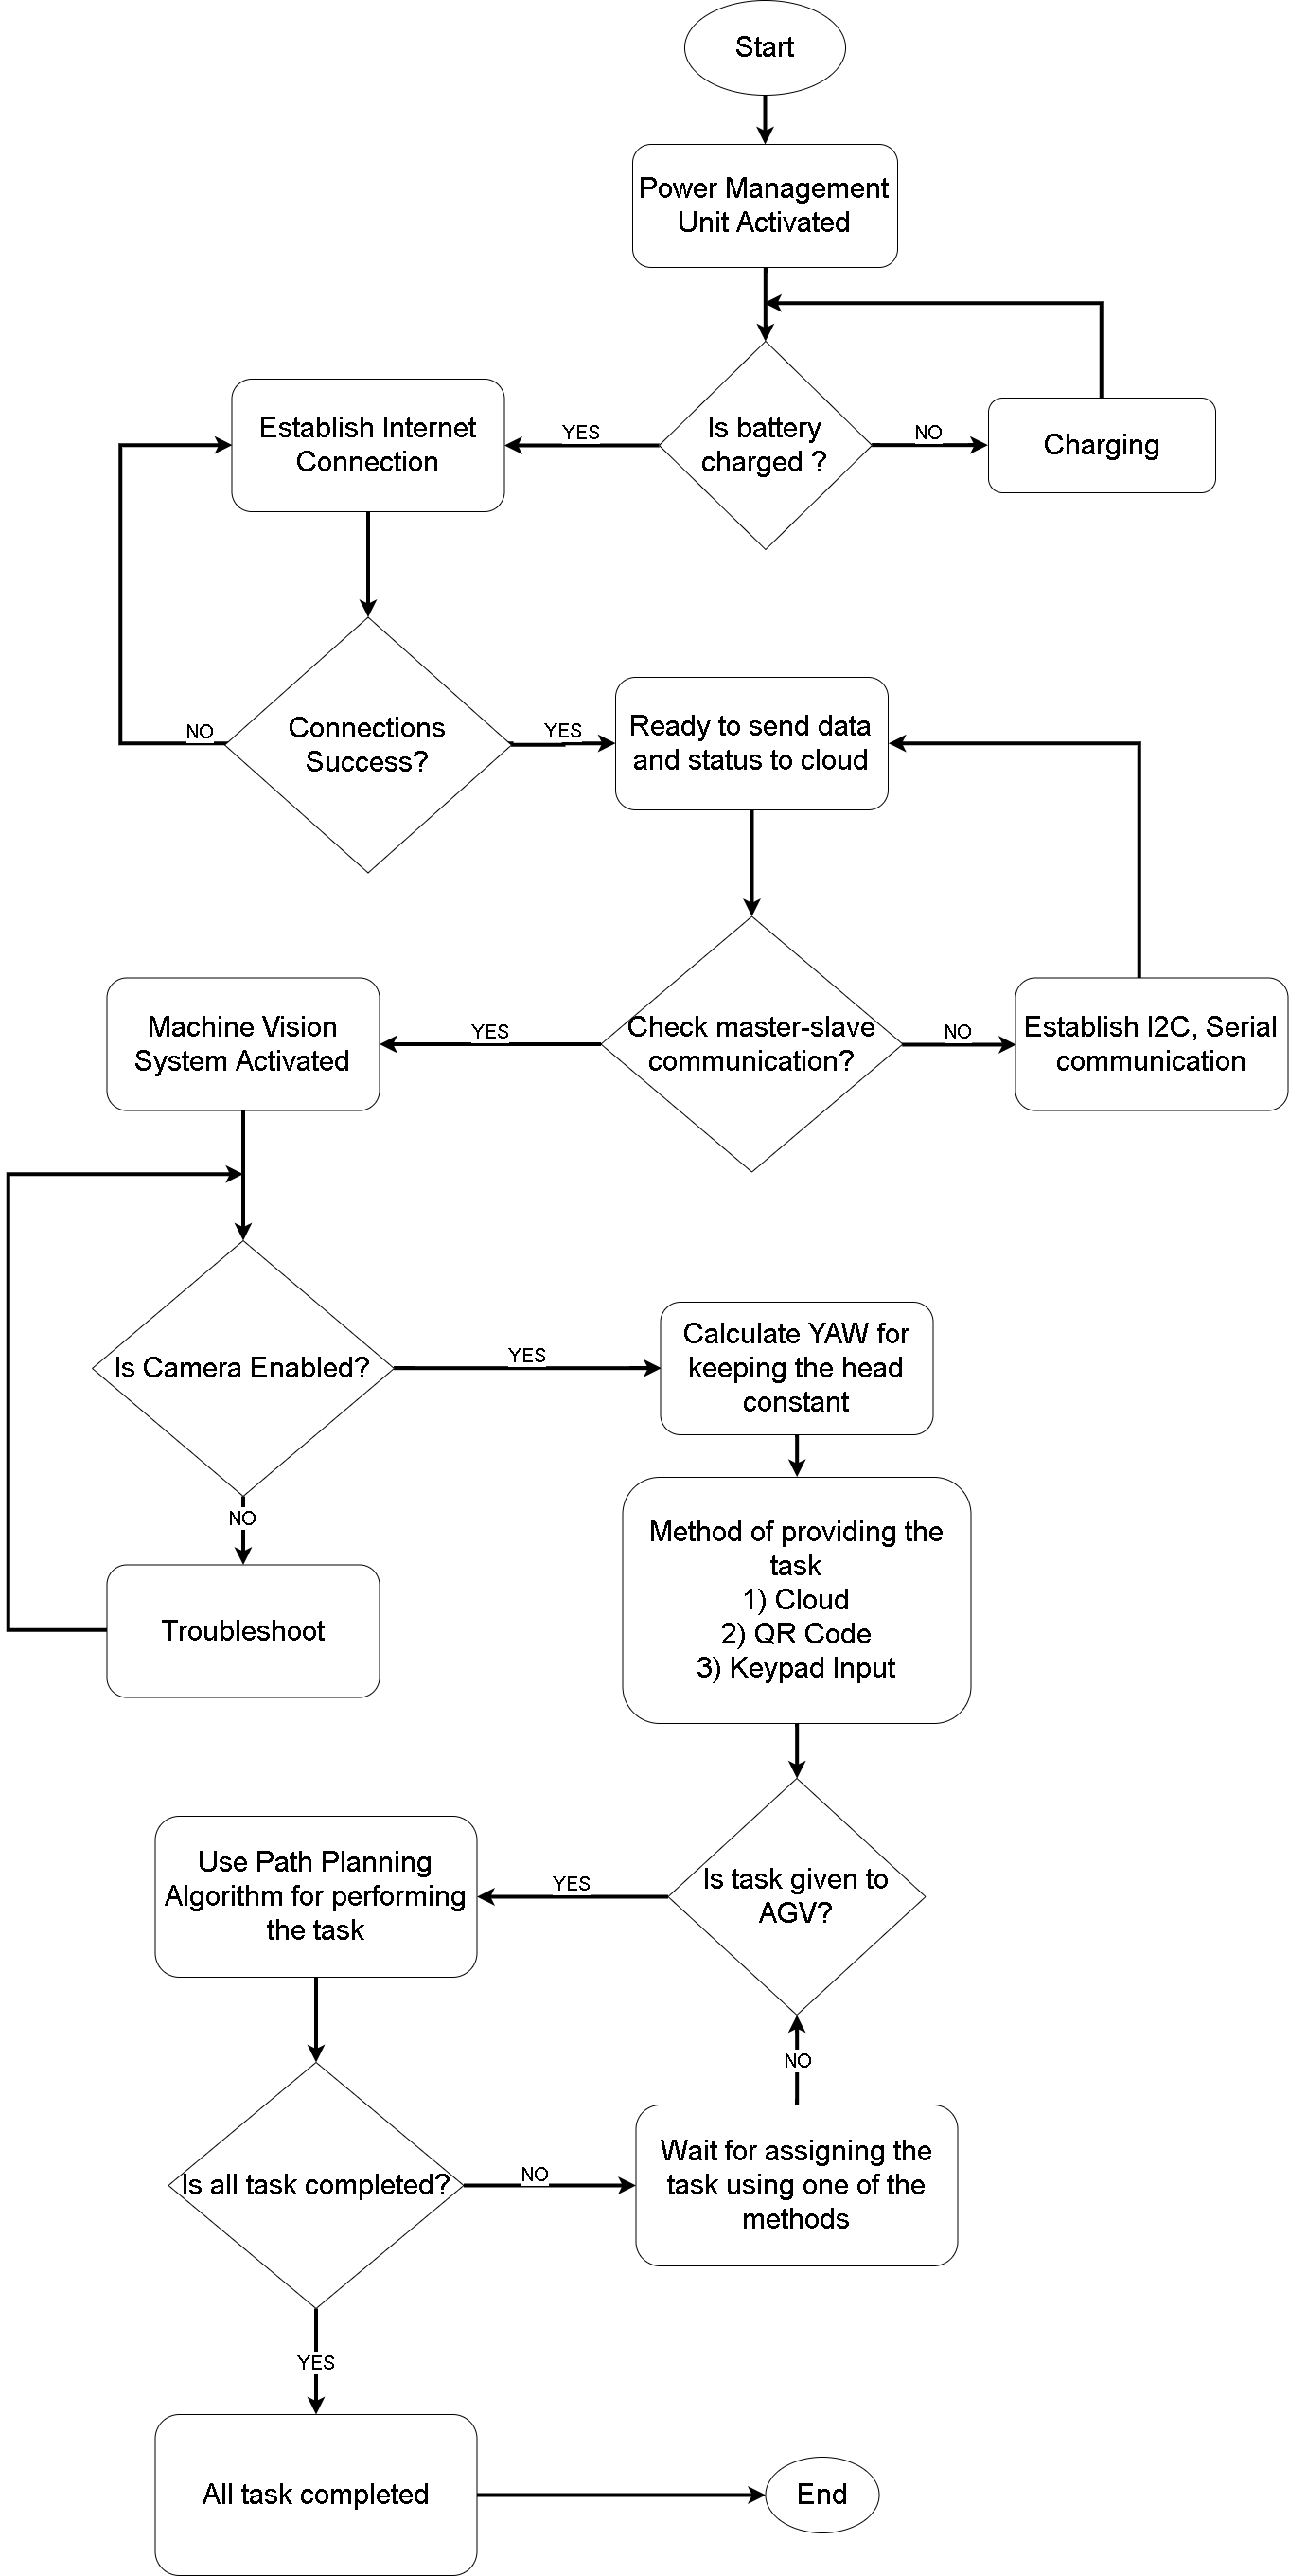
\includegraphics[width=7cm]{Flowchart.png}
\caption{Flow Chart}
\label{fig}
\end{figure}
\newpage
\begin{enumerate}
    \item When AGV is assigned a particular task, firstly it checks whether the battery is charged or not. If it is not AGV will move to the charging station and wait till charging.
    \item Once the battery is checked, AGV establishes an internet connection in order to manage data, and check whether the connection is successful or not.
    \item When all these primary tasks are completed, AGV is ready to perform the assigned task.
    \item In order to perform a task, it needs to check the controller’s communication with slaves. If it is ok the working continues. And if not it establishes necessary communication.
    \item For the movement of proposed AGV, it needs machine vision so, firstly it enables the webcam and necessary hardware successfully. A self-developed path planning algorithm is used for navigation.
    \item The task can be given to AGV through remote accessing using the cloud, QR code or keypad input.
    \item After that, AGV checks whether the assigned task is completed or not if not completed, it waits till the completion of the task and checks for the next task.
\end{enumerate}

\section{Feasibility}

The entire concept of AGVs is based on the system of Flexible Manufacturing Systems (FMS). Machine vision and implementation of ML in AGV provide flexibility by activating operational activities in case of any unpredicted problems and issues including data visualization and analyzation. By automating the battery charging operation, several developments to the AGV technology can be enabled for reducing the charging time of the batteries, leading to a further increase in the efficiency and output of the automation. Our self-developed algorithm and PID- controller assures accuracy and stabilization in navigation respectively.


%\cite{agv_wiki}
%\cite{fujimoto2001}
%\cite{iris2006}
%\cite{grandviewresearch_site}
%\cite{isozaki2011}
%\cite{lozoya2007}
%\cite{piyare2011}
%\cite{cardarelli2015}




\bibliographystyle{plain}
\bibliography{ref}

\end{document}
